\documentclass[journal]{ieee_style}

\usepackage{amsfonts}
\usepackage{minted}
\usepackage{graphicx}
\usepackage{amssymb}
\usepackage{amsmath}
\usepackage{latexsym}
\usepackage{caption}
\usepackage{mathtools}
\usepackage{url}
\usepackage{array}
\usepackage{hyperref}


% correct bad hyphenation here
\hyphenation{op-tical net-works semi-conduc-tor}


\begin{document}
\title{Power-Based Side-Channel Attack for AES Key Extraction on a ATMega328 controller}

\author{Utsav Banerjee,
        Lisa Ho,
        and Skanda Koppula% <-this % stops a space
\thanks{All authors are with the Department
of Electrical and Computer Engineering, Massachusetts Institute of Technology, Cambridge,
MA, 02139 USA}% <-this % stops a space
\thanks{To contact the authors: \texttt{utsav@mit.edu}, \texttt{lisaho@mit.edu}, and \texttt{skandak@mit.edu}}% <-this % stops a space
\thanks{Manuscript completed for 6.858 Computer Systems Security; completed on December 5, 2015}}

\markboth{6.858 Final Project Report - Fall 2015}%
{Power-Based Side-Channel Attack for AES Key Extraction on the ATMega328 controller}
\maketitle

\begin{abstract}
    We demonstrate extraction of a private-key from Flash program memory on the ATMega328 microcontroller (the controller used on the popular Arduino Genuino/Uno board). We loaded a standard AVR-architecture AES implementation onto the chip and ran this implementation to encrypt 500 randomly chosen plaintexts. By carefully measuring the chips power consumption, we were able to correlate the consumed power with the input plaintexts and key values that might be used to encrypt each AES block, and back-derive the hard-coded key used for encryption. We describe here our test infrastructure for automated power trace collection, an overview of our correlation attack, sanitization of the traces and interesting stumbling blocks encountered during data collection and analysis, and the results of our attack.
\end{abstract}

\begin{IEEEkeywords}
AES, side-channel, power consumption, ATMega328, Correlation Power Analysis
\end{IEEEkeywords}

\section{Introduction}
Recent concerns about data privacy has brought attention to the necessity of encryption algorithms. One of the more popular symmetric-key algorithms, Advanced Encryption Standard (AES), has been the U.S. government standard since 2002 (ISO/IEC 18033-3), and is used in a multitude of applications: SSL/TLS protocols \cite{ssl}, Kerberos \cite{kerberos}, and demonstrably secure embedded devices \cite{embedded}. This last application in particular, embedded devices, has seen much growth in recent years, given the advantages of computation on smaller embedded devices: low power, lower system latency, and generally smaller device size.

Small hardware implementations, however, are notoriously vulnerable to a range of side-channel attacks \cite{smalldevice}. Timing, electromagnetic radiation, and power consumption are just three commonly exploited vectors used to leak information about ongoing computations and data on the chip. Knowing that a device architecture is amiable to side-channel exploitation is useful in deciding whether to execute unprotected sensitive computations or store data on devices with similar memory and processor characteristics.

We aim to demonstrate a reasonably realistic side-channel attack on AES on one such embedded device: the ATMega328 microcontroller produced by Atmel. The ATMega328 is the basis for the widely popular development board, Arduino Uno \footnote{Other models of the Arduino, such as the Arduino Mega and Arduino Genuino Micro use ATMega chips as well, that have a similar architecture to the ATMega328. It is possible that this attack could be adapted to those chips as well.}

In section two, we review for the read the theoretical ideas underpinning our attack. In section three, we describe our implementations our hardware setup, power measurement infrastructure, correlation methodologies, instructive problems that we encountered, and overview the structure of our source code. In section four, we describe quantitatively describe the results of our attack.

\section{Preliminaries}
\subsection{Controller Specifications}
The ATMega328 family of chips is an 8-bit microcontroller series with 32 KB of NAND-type flash and 2KB of SRAM. The controller runs off a 16 MHz external clock on the Arduino board. Typical power consumption of the chip ranges from 7 to 12V, with a 20mA current draw, depending on the peripheral and I/O pin usage \cite{atmeldatasheet}. Out attack exploits the NAND-type flash memory architecture that consumes marginally more power when accessing addresses that store value-zero (discharge) bits \footnote{In a highly simplified power consumption model, NAND-flash charges a central power line connected to a series of memory cells. Depending on the value stored in the accessed memory cell, the line is discharged or not. Thus, line requires data-dependent recharging.} \cite{nandflash}.

The encryption program running on our ATMega328 uses an Arduino-specific port of the \texttt{avr-crypto-lib} by Davy Landman and Bochum Hackerspace \cite{AESLib} \cite{daslabor}. \texttt{AESLib} is one of the more widely-used AES implementations for Arduino, and includes support for ECB and CBC-modes of AES. Our team decided that ECB-mode would be more amiable to a power correlation attack, and correspondingly chose to exploit the library's AES-ECB implementation. We discuss ECB in further depth in section 3.D.

\subsection{Correlation Power Analysis}
% Briefly explain how CPA works
% sbox, AES is a block cipher that encrypts blocks of plaintext in a number 

\section{Protocols and Procedure}
\subsection{Data Collection Infrastructure}
A central piece of our work was developing the serial-connection based data collection framework to feed plaintexts for encryption to the Arduino, and read the resulting power trace from the oscilloscope. An outline is given in Figure 1.

\begin{figure}[!t]
\centering
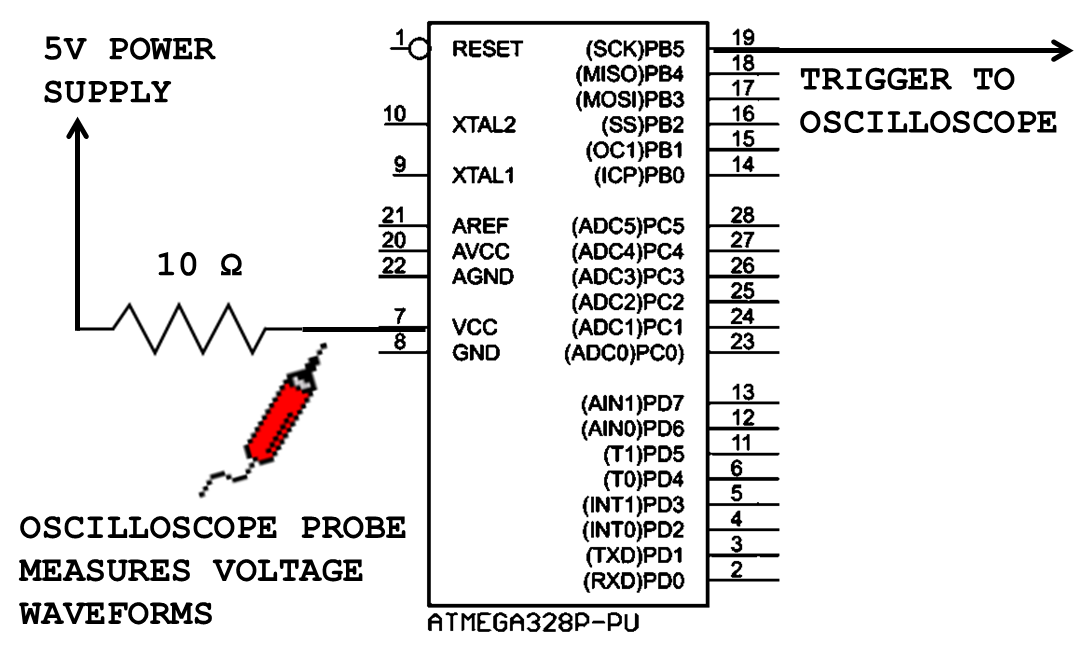
\includegraphics[width=2.5in]{Experiment_Setup}
\caption{The oscilloscope probes voltages on the chip's power line, starting automated power trace on a trigger that signals the start of AES}
\label{fig_sim}
\end{figure}

We needed a subset of the power trace that correlated strongly with the input plaintext and key. Specifically, we were interested in finding the portion of the trace that corresponded to the \texttt{xor(plaintext,key)} operation, and the the SBOX permutation taken over the \texttt{xor} result. In order to automate slicing to this part of the trace, we modified the \texttt{AESLib} SBOX assembly code to insert a flag a memory-mapped register that pulled up pin 13. Our oscilloscope triggered on this output, and automatically captured the part of the trace immediately after the pin 13 rising edge. 

Central to our collection was a Tektronix 5054B computing oscilloscope that collected samples at 4GHz with internal memory bank of at most 16 million points. The sampling rate limited the resolution of traces that we were able to capture; we originally thought this physical cap on data quality was causing correlation issues we ran into, until we discovered arbitrary DC shifts in the traces. We discuss this challenge in more detail in Section 3.C. We used the oscilloscope's GPIB query interface to automate configuration and downloading of traces.

In the final iteration of our system, we have a orchestrating computer $C$ send plaintexts to the Arduino for encryption every 2 seconds over the Arduino's serial port. The pin 13 trigger resulting in a oscilloscope trace capture, which was sent back to $C$. 

More recently, we have been attempting to use the Tektronix $Fast Frames$ feature to take capture batches of 2,500-point traces at once, and use one memory-read, GPIB-write operation to transfer these traces to the computer. This would allow us much faster trace measurement, which is currently bottlenecked by the GPIB-write operation. As we will discuss in Section 4, the number of key bytes we can recover is directly correlated with the number of plaintexts we can capture and average.

Photos of our collection framework can be found at \texttt{\url{https://www.dropbox.com/sh/usialgelvfqlsdr/AACvqOHKEWoumWNYi2WRIebCa?dl=0}}. Of perhaps small interest is the grounded aluminum food box encapsulating the ATMega328 setup, which reduced the EM noise and interference which we noticed in our power traces.

\subsection{Implementation of CPA and Power Model}
- discuss different power models we've tried, faster correlation

\subsection{Instructive Problems Encountered (and Panaceas)}


\begin{itemize}[-]
\item remove difAmp -> increase resistor value -> increase bandwidth?//used to measure current before
\item serial print adds noise
\item averaging to solve dc shift
\item interrupt introduces clock jitter
\item adding nops to prevent asyncronous / delay
\item original hypothesis about sbox:  SBox bad for correlation? the flash architecture -> bit block bit block bar
\item FUNDAMENTALLY A PROBLEM WITH DATA
\end{itemize}
\subsection{Caveats}
We address concerns and discuss the drawbacks for our chosen method of attack:
\begin{itemize}
    \item[--] We chose to attack the Arduino library's implementation AES-ECB mode. Althought ECB is not semantically secure (e.g. you can derive information about the plaintext from the ciphertext), ECB is still (unfortunately) used as the default option in a number of crypto-suites, \texttt{avr-crypto-lib} included. This is because of it's relatively simple implementation, compared to other more sophisticated modes of AES. Furthermore, our attack does not exploit the plaintext-ciphertext correlations in ECB to derive the key; rather, it uses our power sidechannel. For our team's first power-trace based attack, we chose a mode that we were confident that might have some correlation with the plaintext-key-guess XOR (the first computation in the first step of ECB). It might be possible to adapt our attack to CBC-mode as well.
- presence of trigger
- more
- go over the graphs, and timing/accuracy results of tests
\end{itemize}
\subsection{Overview of Source Code}
- overview everything in dropbox

\section{Results}
2.5 hours for 500 plaintexts
5 minutes to process

Most of our data and results can be found at \texttt{\url{https://www.dropbox.com/sh/07xni6s4tu4klme/AABnrBK-QZCVO1tMK4GFeQ5ta?dl=0}}.

\section*{Acknowledgment}
The authors would like to extend our deepest thanks to Chiraag Juvekar of the Energy Efficient Digital Circuits and Systems group for the time he spent with us aiding our debugging of data collection and analysis problems. We would also like to thank Albert Kwon, our TA, for his insightful advice over the course of the project.


\begin{thebibliography}{1}
\bibitem{ssl}
Lee, Homin K and Malkin, Tal and Nahum, Erich, \emph{Cryptographic strength of ssl/tls servers: current and recent practices}.\hskip 1em plus
  0.5em minus 0.4em\relax Proceedings of the 7th ACM SIGCOMM conference on Internet measurement, 2007.

\bibitem{kerberos}
Rathore, Romendrapal Singh and Pal, BL and Kumar, Shiv. \emph{Analysis and Improvement in Kerberos 5}.\hskip 1em plus
  0.5em minus 0.4em\relax 2015.

\bibitem{embedded}
Altera Corporation, \emph{FPGAs with built-in AES: The key to secure system designs}.\hskip 1em plus
  0.5em minus 0.4em\relax Embedded Computing Design, July 15, 2008.

\bibitem{smalldevice}
Oswald, Elisabeth, et al.  \emph{Side-Channel Analysis Resistant Description of the AES S-Box}.\hskip 1em plus 
  0.5em minus 0.4em\relax 2005.

\bibitem{AESLib}
    \url{https://github.com/DavyLandman/AESLib}. \emph{Arduino AESLib}. \hskip 1em plus
    0.5em minus 0.4em\relax 2015.

\bibitem{daslabor}
    \url{http://www.das-labor.org/wiki/AVR-Crypto-Lib/en}. \emph{AVR-Crypto-Lib}. \hskip 1em plus
    0.5em minus 0.4em\relax 2013.

\bibitem{atmeldatasheet}
    \url{http://goo.gl/hhZF2z}. \emph{Atmel 8-bit Microcontroller Datasheet}. \hskip 1em plus
    0.5em minus 0.4em\relax 2014.

\bibitem{nandflash}
    Handy, Jim. \url{http://goo.gl/5QZHhK} \emph{3D NAND: Making a Vertical String}. \hskip 1em plus
    0.5em minus 0.4em\relax 2013.
\end{thebibliography}
\end{document}


